\documentclass[12pt, twoside]{book}
\usepackage[a4paper,width=150mm,top=25mm,bottom=25mm,bindingoffset=6mm]{geometry}
\usepackage[utf8]{inputenc}
\usepackage[italian]{babel}
\usepackage{caption}
\usepackage{fancyhdr}
\usepackage{newlfont}
\usepackage{float}
\usepackage{xcolor}
\usepackage[nottoc]{tocbibind}
\usepackage{emptypage}
\usepackage{titlesec}
\usepackage[T1]{fontenc}
\usepackage{blindtext, array}
\usepackage[sorting=none,backend=bibtex]{biblatex}
\usepackage{csquotes}
\usepackage{pdfpages}
\usepackage{listings}
\usepackage{amsmath}
\usepackage[cache=false]{minted}
\usepackage{setspace}
\usepackage[hidelinks]{hyperref}
\usepackage{outline}
\usepackage{enumitem}
\usepackage{mathtools}
\usepackage{xparse}
\usepackage{svg}
\usepackage{tikz}
\usepackage{lipsum}
\usepackage[toc,page]{appendix}
\usepackage{amsfonts}
\usepackage{subcaption}
\usepackage[htt]{hyphenat}
\usetikzlibrary{shapes.geometric, arrows, positioning}


%%%%%%%%%%%%%%%%%%%%%%%%%%%%%%%%%%%%%%%%%%%%%%%
\setlist{nosep}

% Stile di pagina
% \pagestyle{fancy}
\usemintedstyle{colorful}

\definecolor{lightgray}{gray}{0.95}

% Stile dei titoli dei capitoli
\definecolor{gray75}{gray}{0.75}
\newcommand{\hsp}{\hspace{20pt}}
\titleformat{\chapter}[hang]
{\Huge\bfseries}
{\thechapter\hsp\textcolor{gray75}{|}\hsp}
{0pt}
{\Huge\bfseries}

% lnorm command
\DeclarePairedDelimiter{\norm}{\lVert}{\rVert}

\newenvironment{equationderivation}[1][]{%
    \begin{trivlist}%
    \item[]\textbf{Passaggi #1:}%
}{%
    \end{trivlist}%
}

\newenvironment{proof}[1][]{%
    \begin{trivlist}%
    \item[]\textbf{Dimostrazione #1:}%
}{%
    \end{trivlist}%
}

% \raggedbottom
%%%%%%%%%%%%%%%%%%%%%%%%%%%%%%%%%%%%%%%%%%%%%%%

% Bibliografia
\addbibresource{bibliografia.bib}

\onehalfspacing
\begin{document}

\begin{titlepage}
    \begin{center}
        {{\Large{\textsc{Alma Mater Studiorum $\cdot$ Universit\`a di Bologna}}}}
        \rule[0.1cm]{15cm}{0.1mm}
        \rule[0.5cm]{15cm}{0.6mm}
        \\\vspace{3mm}
        {\small{\bf Scuola di Ingegneria e Architettura \\
                Dipartimento di Informatica $\cdot$ Scienza e Ingegneria $\cdot$ DISI\\
                Corso di Laurea Magistrale in Ingegneria Informatica}}
    \end{center}

    \vspace{23mm}

    \begin{center}{
            \large \bf GoDP: una nuova soluzione per la gestione e la differential privacy dei dati sensibili \par
        }\end{center}
    \vspace{40mm} \par \noindent
    \begin{minipage}[t]{0.47\textwidth}{
        \large{Relatore:
        \vspace{2mm}\\
        {\bf Prof. Michele Colajanni}
        }
        \vspace{4mm}\\
        \large{Correlatore:
        \vspace{2mm}\\
        {\bf Ing. Silvio Russo}
        }
    }
    \end{minipage}
    %
    \hfill
    %
    \begin{minipage}[t]{0.47\textwidth}\raggedleft{
            {\large{Presentata da:
                        \vspace{2mm}\\
                        \bf Riccardo Barbieri}}}
    \end{minipage}
    \vspace{40mm}
    \begin{center}
        Anno Accademico 2023/2024
    \end{center}
\end{titlepage}

\phantomsection
\listoffigures

\tableofcontents

\chapter*{Introduzione}
---\textit{Ancora un placeholder, da modificare}---
La privacy dei dati è diventata una preoccupazione sempre più importante nell'era digitale. Con la crescente raccolta e l'analisi di dati personali, è fondamentale garantire che le informazioni individuali siano protette da accessi non autorizzati e da usi impropri. La privacy differenziale (DP) è una rigorosa definizione matematica di privacy che offre forti garanzie di riservatezza anche quando i dati vengono utilizzati per l'analisi.


\chapter{Stato dell'arte}

\section{Introduzione alla Differential Privacy}
La privacy differenziale (DP) è un rigoroso framework matematico per la progettazione di algoritmi utilizzati per la creazione di distribuzioni di dati aggregati su dataset; gli algoritmi che rispettano la definizione di DP sono in grado di limitare l'impatto che la partecipazione di un singolo individuo ha sui risultati dell'analisi aggiungendo una ragionevole quantità di rumore casuale, rendendo \textit{quasi} impossibile confermare o negare la presenza di un soggetto all'interno del dataset utilizzato per l'aggregazione di dati. Questa proprietà è cruciale per prevenire che eventuali attaccanti possano inferire informazioni sensibili su individui partecipanti al dataset, anche in presenza di informazioni ausiliari.

La motivazione alla base della privacy differenziale deriva dalla necessità di bilanciare l'utilità dei dati con la protezione della privacy in un mondo sempre più incentrato sui dati. Con la proliferazione di machine learning, big data e generale condivisione di dati, le tecniche di anonimizzazione tradizionali si sono rivelate inadeguate. Queste tecniche falliscono nel garantire privacy ai soggetti di un dataset a causa della disponibilità di dati da fonti come social network \cite{deanon-socialnet}, piattaforme di streaming \cite{deanon-netflix} e dispositivi di geo-localizzazione \cite{deanon-geodata}, permettendo a un attaccante di associare dati sensibili agli individui.

\section{Contesto storico}
Il concetto di privacy differenziale (DP) è stato introdotto formalmente da Cynthia Dwork \cite{10.1007/11681878_14}, dove viene formalizzata la definizione di $\varepsilon$-privacy differenziale e dimostrato come l'aggiunta di rumore calibrato alla sensitività di una funzione possa proteggere la privacy individuale mantenendo un certo grado di utilità dei dati.

\subsection{Metodi tradizionali per la protezione della privacy}
Prima dell'avvento della privacy differenziale, l'anonimizzazione dei dati si basava su tecniche come k-anonimity, l-diversity e t-closeness; questi metodi sono in grado di prevenire la re-identificazione dei soggetti senza limitare la divulgazione dei singoli valori degli attributi, imponendo regole sulla distribuzione e quantità di valori distinti degli attributi rilasciati. Queste tecniche permettono di creare distribuzioni di dati che, prese da sole, garantiscono un alto livello di privacy; sono tuttavia vulnerabili ad attacchi che sfruttano informazioni ausiliarie.

Dato che un editore di dati non è in grado di controllare quali informazioni aggiuntive verranno rilasciate in futuro sui partecipanti ai propri dataset, la privacy differenziale costituisce una soluzione ideale rispetto ai metodi tradizionali, data la particolare resistenza agli attacchi che si basano sulla disponibilità di informazioni aggiuntive.

Un'altra differenza fondamentale che la privacy differenziale presenta rispetto a metodi tradizionali è la possibilità di quantificare il livello di privacy perso con una distribuzione di dati tramite un apposito parametro; questa caratteristica permette di stabilire e tracciare un budget di privacy per uno specifico dataset al contrario dei metodi tradizionali sopra citati.

\section{Utilizzi privacy differenziale}
Il framework della privacy differenziale è stato adottato in diversi ambiti, a partire dall'analisi lessicale per sistemi di suggerimenti per tastiere alla raccolta di informazioni sull'utilizzo di piattaforme web; di seguito verranno documentati alcuni esempi.

Apple utilizza la privacy differenziale con modello locale per anonimizzare i dati raccolti da dispositivi iOS e macOS; questi dati vengono utilizzati per migliorare le funzionalità di suggerimenti per tastiera e identificazione di siti web che causano interruzioni o altri errori al browser Safari \cite{appledpatscale}.

Google ha utilizzato la privacy differenziale in svariati contesti, in particolare ha spesso utilizzato il framework per analisi dall'enorme mole di dati GPS ottenuti dai dispositivi con un account Google. Una di queste analisi, Community Mobility Reports, nasce per quantificare cambiamenti in pattern di mobilità durante la pandemia COVID-19: qui la privacy differenziale permette di non pubblicare mai valori assoluti sulle visite \cite{googlecovid19communitymobility}.

La Audience Engagements API di Linkedin costituisce un altro interessante esempio di applicazione del framework perché si tratta di un'implementazione del modello distribuito interattivo: diversamente dagli esempi precedenti il rilascio dei dati non avviene tutto contemporaneamente, un \textit{analista} richiede i dati di cui necessita in modo incrementale; questo sistema impone limitazioni nella quantità di dati accessibili in un dato periodo per poter garantire un certo livello di anonimizzazione \cite{rogers2020linkedinsaudienceengagementsapi}.

\section{Privacy differenziale e machine learning}
Negli ultimi anni, modelli di machine learning vengono dispiegati sempre più spesso in ambiti che hanno a che fare con domini sensibili come sanità, finanza e social network, che spesso forniscono dati che contengono informazioni riservate. L'allenamento di modelli ML su dati sensibili può portare, durante il loro utilizzo, alla fuoriuscita di questi dati \cite{Zhang_2023mlprivacy} sfruttando tecniche come model inversion \cite{OWASPmlinversion:online} e membership inference \cite{OWASPmembinference:online}; queste vulnerabilità presentano un rischio significativo per la privacy degli individui e per la sicurezza delle organizzazioni che gestiscono tali dati.

Per sopperire a queste vulnerabilità, sono state sviluppate diverse tecniche che incorporano la privacy differenziale durante l'addestramento o durante l'inferenza sui dati.

\subsection{Differentially Private Stochastic Gradient Descent}

Uno dei primi esempi di questi metodi è la tecnica \textit{Differentially Private Stochastic Gradient Descent} che consiste in una variante dell'algoritmo SGD standard che prevede l'aggiunta di rumore accuratamente calibrato ai gradienti a ogni iterazione del processo di addestramento così come la limitazione degli stessi per limitare la loro sensitività \cite{Abadi_2016dpsgd}; questa tecnica è usata per addestrare modelli di deep learning.

\subsection{Private Aggregation of Teacher Ensembles}

Un altro approccio a questo problema nell'ambito della classificazione è \textit{Private Aggregation of Teacher Ensembles}, tecnica che addestra un modello \textit{studente} utilizzando i dati forniti da un insieme di modelli \textit{insegnanti} addestrati su set disgiunti del dataset iniziale; l'output fornito dall'insieme di insegnanti è reso privato con l'aggiunta di rumore opportunamente calibrato \cite{papernot2018scalableprivatelearningpate}.

\subsection{Private Federated Learning}
L'approccio di federated learning consente di allenare un modello di machine learning in maniera distribuita, senza dover condividere i dati utilizzati per l'addestramento; i client condividono il risultato dell'allenamento con un server centrale che agisce da aggregatore creando un unico modello.

Questa tecnica da sola garantisce un certo livello di privacy nei dati dato che non è necessario che l'aggregatore abbia accesso al dataset completo; le garanzie di privacy di questo modello possono tuttavia essere migliorate condividendo gli aggiornamenti dei modelli locali al server dopo averli mascherati con un algoritmo differenzialmente privato. Il rumore aggiunto assicura che la contribuzione di una singola voce del dataset non possa essere inferita facilmente \cite{peterson2019privatefederatedlearningdomain}.

\section{Strumenti per la privacy differenziale}
Negli ultimi anni sono nati vari strumenti per permettere a utenti non tecnici di creare release di dati protette dalle garanzie offerte dalla privacy differenziale.

Nell'ambito open source, i framework più utilizzati sono OpenDP e le Google Differential Privacy Libraries.

Uno degli strumenti più diffusi è \textit{OpenDP}, una libreria open source sviluppata dall'Harvard University, che fornisce una suite di algoritmi per l'analisi statistica, ed è basata parzialmente sulle librerie di Google. Offre implementazioni in Rust e Python così come un'interfaccia SQL per integrare la libreria con workflow esistenti \cite{opendp}.

Le librerie di Google sono un insieme di strumenti per realizzare applicazioni che includono l'utilizzo della privacy differenziale; Google fornisce una libreria di elementi base in Go, Java e C++ che include le primitive per realizzare aggregazioni differenzialmente private per l'aggiunta di rumore calibrato.\\
Questi elementi costituiscono la base del framework Privacy on Beam, un framework che integra tecniche di privacy differenziale all'interno di pipeline di elaborazione dati composte con Apache Beam.\\
In questo pacchetto di Google sono inclusi anche componenti per la gestione del budget della privacy e per effettuare verifiche formali sulle garanzie offerte dalla privacy differenziale.

Passando a strumenti enterprise, Tumult Labs propone una soluzione per applicazioni industriali ad alta scalabilità basata su Apache Spark distribuita sotto forma di una libreria Python. Offrono soluzioni mirate al settore pubblico nel rispetto delle normative vigenti e al settore finanziario \cite{tumultanalytics}.

In questo lavoro di tesi si mira a creare uno strumento basato su Privacy on Beam con l'obiettivo di sviluppare una soluzione che consenta la creazione di release di dati differenzialmente private di piccoli-medi dataset tramite una semplice interfaccia da linea di comando e file di configurazione. Questo strumento è pensato per essere adatto a progetti di piccola entità, ad esempio per semplificare la creazione di release di dati per gruppi di ricerca, piccoli media outlet o interne a un'azienda.








\chapter{Meccanismi Differenzialmente Privati}


\section{Definizione}
La definizione seguente costituisce un formalismo più ristretto rispetto alla definizione completa, quest'ultima include un secondo parametro $\mathcal{\delta}$, la cui funzione e utilità verranno discusse in seguito.

Una trasformazione $\mathcal{M}$ è considerata $\varepsilon$-differenzialmente privata se, per ogni dataset $D_1$ e $D_2$ che differiscono al massimo per un individuo ($\norm{D_1 - D_2}_1 \le 1$) e ogni $S \subseteq \operatorname{Range}(\mathcal{M})$, vale la seguente disequazione \cite{10.1007/11681878_14}:
\begin{equation}
  \Pr[\mathcal{M}(D_1) = S] \le e^{\varepsilon} \cdot \Pr[\mathcal{M}(D_2) = S]
  \label{eq:e_differential_privacy}
\end{equation}

I termini $\Pr[\mathcal{M}(D_1) = S]$ e $\Pr[\mathcal{M}(D_2) = S]$ indicano la probabilità che il risultato dell'applicazione del meccanismo $\mathcal{M}$ su $D_1$ e $D_2$ risulti nell'output $S \in \operatorname{Range}(\mathcal{M})$.
Il termine $e^\varepsilon, \varepsilon > 0$ rappresenta un coefficiente che indica quanto le due probabilità possono differire tra di loro, in particolare per valori di $\varepsilon$ vicini a $0$ le probabilità sono simili; all'aumentare di $\varepsilon$ la differenza tra le due probabilità può aumentare.

Considerando che i due database $D_1$ e $D_2$ differiscono per un solo individuo, essi sono intercambiabili; ciò rende la definizione simmetrica. Vale quindi anche:
\begin{equation}
  e^{-\varepsilon} \cdot \Pr[\mathcal{M}(D_2) = S] \le \Pr[\mathcal{M}(D_1) = S] \le e^{\varepsilon} \cdot \Pr[\mathcal{M}(D_2) = S]
  \label{eq:e_differential_privacy_symm}
\end{equation}

\subsubsection{Un esempio pratico}
\label{ex:coint_toss}
Si supponga di volere condurre un sondaggio su una popolazione ponendo la domanda: "Nell'ultimo anno hai guidato un veicolo sotto l'influenza di alcol o stupefacenti?".
Ovviamente, una persona alla quale viene posta direttamente questa domanda tenderà a mentire allo scopo di proteggere la propria privacy e evitare di auto incriminarsi. In questa istanza può rendersi utile l'applicazione di un meccanismo differenzialmente privato.

Per ovviare a questa limitazione del processo di raccolta dati, si richiede ai partecipanti di lanciare una moneta senza mostrare il risultato:
\begin{itemize}
    \item se il risultato è testa il soggetto risponde alla domanda in modo sincero
    \item se il risultato è croce il soggetto lancia una seconda moneta: su testa risponde "Si", su croce "No"
\end{itemize}

\begin{tikzpicture}
\node (start) [draw,font=\scriptsize,rectangle,align=center,text width=0.2*\textwidth] {Nell'ultimo anno hai guidato un veicolo sotto l'influenza di alcol o stupefacenti?};

\node (dec1) [draw,font=\scriptsize,rectangle,right=2.5cm of start.center] {Lancia moneta};
\node (heads1) [draw,minimum height=1cm,minimum width=1cm,font=\scriptsize,circle,above=1cm of dec1.center] {Testa};
\node (tails1) [draw,minimum height=1cm,minimum width=1cm,font=\scriptsize,circle,below=1cm of dec1.center] {Croce};

\node (heads2) [draw,minimum height=1cm,minimum width=1cm,font=\scriptsize,circle,right=2cm of dec1.center] {Testa};
\node (truth) [draw,font=\scriptsize,rectangle,above=of heads2.north,right=2cm of heads1.center] {Verità};
\node (dec2) [draw,font=\scriptsize,rectangle,below=of heads2.south,right=2cm of tails1.east,anchor=center] {Lancia moneta};

\node (tails2) [draw,minimum height=1cm,minimum width=1cm,font=\scriptsize,circle,right=1cm of dec2.east] {Croce};
\node (out1) [draw,font=\scriptsize,rectangle,above=of tails2.north,right=of heads2.east] {Rispondi "Si"};
\node (out2) [draw,font=\scriptsize,rectangle,right=1cm of tails2.east] {Rispondi "No"};

\draw [-latex] (start.east) -- (dec1.west);
\draw [-latex] (dec1.north) -- (heads1.south);
\draw [-latex] (dec1.south) -- (tails1.north);
\draw [-latex] (tails1.east) -- (dec2.west);
\draw [-latex] (heads1.east) -- (truth.west);
\draw [-latex] (dec2.north) -- (heads2.south);
\draw [-latex] (dec2.east) -- (tails2.west);
\draw [-latex] (tails2.east) -- (out2.west);
\draw [-latex] (heads2.east) -- (out1.west);
\end{tikzpicture}

Questo processo introduce un elemento casuale alla risposta di un singolo soggetto, offrendo all'individuo una negazione plausibile contro eventuali accuse e impedendo a terze parti di discriminare sulla base delle risposte \cite{Warner01031965}.

Nel complesso, riscrivendo i risultati nei termini della definizione si ottiene:
\begin{itemize}
    \item $\Pr[\mathcal{M}(Si) = Si] = 0.75$, $\Pr[\mathcal{M}(Si) = No] = 0.25$
    \item $\Pr[\mathcal{M}(No) = Si] = 0.25$, $\Pr[\mathcal{M}(No) = No] = 0.75$
\end{itemize}

Considerati questi risultati si può affermare che il meccanismo illustrato è $\ln{3}$-differenzialmente privato; si può dimostrare partendo dalla definizione \eqref{eq:e_differential_privacy} che:
\begin{align*}
    \frac{\Pr[\mathcal{M}(D_1) = S]}{\Pr[\mathcal{M}(D_2) = S]
    } &\le e^{\varepsilon}\\
    \frac{\Pr[\mathcal{M}(Si) = Si]}{\Pr[\mathcal{M}(Si) = No]} &\le 3 = \frac{\Pr[\mathcal{M}(No) = No]}{\Pr[\mathcal{M}(No) = Si]}
\end{align*}

Il meccanismo illustrato dimostra in termini semplici come la privacy differenziale possa agire sui dati per proteggere la privacy dei partecipanti che aderiscono a essere inseriti in una raccolta di dati. Come specificato in precedenza, questo processo garantisce negazione plausibile sul contenuto della risposta ai soggetti partecipanti; non fornisce tuttavia la possibilità di negare di aver partecipato al sondaggio. Al contrario, la privacy differenziale è applicabile solamente a distribuzioni di dati basate su sistemi di interrogazione che generano risultati aggregati.

\subsection{Quantificazione della conoscenza dell'attaccante}
Il parametro $\varepsilon$ presente nella definizione di $\varepsilon$-DP può essere interpretato come una misura del livello massimo di conoscenza che un potenziale attaccante può guadagnare osservando i risultati di un'interrogazione del meccanismo differenzialmente privato.

Prendendo come riferimento un attaccante che conosce l'intero database eccetto il soggetto target si può modellare il suo punto di vista considerando due possibili dataset: $D_{in}$ contiene il target mentre $D_{out}$ no; l'obiettivo dell'attaccante è capire quale dei due database è quello reale.

Nel modello dell'attaccante si può esprimere il sospetto che il database $D$ sia $D_{in}$ come $\Pr[D = D_{in}] = 1 - \Pr[D = D_{out}]$. Si supponga ora che l'attaccante abbia osservato che il meccanismo DP applicato a $D$ restituisce l'output $O$: si può esprimere la probabilità che $D = D_{in}$ dopo aver osservato l'output come $\Pr[D = D_{in} | \mathcal{M}(D) = O]$; applicando il teorema di Bayes si ottiene un'espressione che permette di quantificare il livello di sospetto $Pr[D = D_{in}|M(D) = O]$ che l'attaccante ha dopo aver osservato l'output $O$.
\begin{equation}
\label{eq:bayes_susp}
    \Pr[D = D_{in} | \mathcal{M}(D) = O] = \frac{\Pr[D = D_{in}] \cdot \Pr[\mathcal{M}(D) = O | D = D_{in}]}{\Pr[\mathcal{M}(D) = O]}
\end{equation}
Il termine $\Pr[D = D_{in}]$ è il sospetto iniziale e il termine $\Pr[\mathcal{M}(D) = O | D = D_{in}]$ può essere riscritto come $\Pr[\mathcal{M}(D_{in}) = O]$ indicando la probabilità che il meccanismo $\mathcal{M}$ applicato a $D_{in}$ restituisca $O$. Mentre i primi due termini sono conosciuti, il termine $\Pr[\mathcal{M}(D) = O]$ è sconosciuto; per rimediare si può considerare il rapporto tra i due sospetti aggiornati all'output $O$.
\begin{equation}
\label{eq:bayes_susp_ratio}
    \frac{\Pr[D = D_{in} | \mathcal{M}(D) = O]}{\Pr[D = D_{out} | \mathcal{M}(D) = O]} = \frac{\Pr[D = D_{in}]}{\Pr[D = D_{out}]} \cdot \frac{\Pr[\mathcal{M}(D_{in}) = O]}{\Pr[\mathcal{M}(D_{out}) = O]}
\end{equation}
In questa espressione emerge il termine $\frac{\Pr[\mathcal{M}(D_{in}) = O]}{\Pr[\mathcal{M}(D_{out}) = O]}$, la definizione di $\varepsilon$-DP \eqref{eq:e_differential_privacy} limita il rapporto come segue:
\begin{equation}
\label{eq:e_dp_bounds}
    e^{-\varepsilon} \le \frac{\Pr[\mathcal{M}(D_{in}) = O]}{\Pr[\mathcal{M}(D_{out}) = O]} \le e^{\varepsilon}
\end{equation}
Applicando all'equazione \eqref{eq:bayes_susp_ratio} si ottiene:
\begin{equation}
\label{eq:mid_information_gain}
    e^{-\varepsilon} \cdot \frac{\Pr[D = D_{in}]}{\Pr[D = D_{out}]} \le \frac{\Pr[D = D_{in} | \mathcal{M}(D) = O]}{\Pr[D = D_{out} | \mathcal{M}(D) = O]} \le e^{\varepsilon} \cdot \frac{\Pr[D = D_{in}]}{\Pr[D = D_{out}]} 
\end{equation}
Applicando le sostituzioni $\Pr[D = D_{out}] = 1 - \Pr[D = D_{in}]$ e $\Pr[D = D_{out} | \mathcal{M}(D) = O] = 1 - \Pr[D = D_{in} | \mathcal{M}(D) = O]$ e riorganizzando i termini si ottiene:
\begin{equation}
\label{eq:information_gain}
    \frac{\Pr[D = D_{in}]}{e^\varepsilon + (1 - e^\varepsilon) \cdot \Pr[D = D_{in}]} \le \Pr[D = D_{in} | \mathcal{M}(D) = O] \le \frac{e^\varepsilon \cdot \Pr[D = D_{in}]}{1 + (e^\varepsilon - 1) \cdot \Pr[D = D_{in}]}
\end{equation}
Per i passaggi della trasformazione, consultare l'appendice \ref{eqd:information_gain_derivation}.

Tracciando il grafico dell'espressione risultante al variare di $\varepsilon$ si può notare come il guadagno di informazione potenziale possa aumentare drasticamente per valori di $\varepsilon$ alti.
\begin{figure}[H]
    \centering
    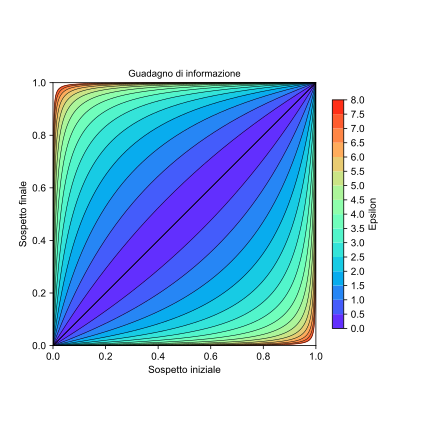
\includegraphics[scale=0.8]{plots/information_gain.pdf}
    \caption{Guadagno di informazione sul dataset al variare di epsilon}
\end{figure}

\section{Meccanismo di Laplace}
Le query più comuni che vengono effettuate su database sono di tipo numerico, precisamente sono funzioni del tipo $f \colon \mathbb{N}^{|\mathcal{X}|} \to \mathbb{R}^k$, dove $\mathcal{X}$ rappresenta l'universo di possibili record in un database $x$.

Per rendere questa tipologia di query differenzialmente privata con il meccanismo di Laplace si aggiunge rumore campionato da una distribuzione di Laplace:
\begin{align}
\label{eq:laplace_distribution}
    Lap(x|\mu,b) = \frac{1}{2b}\exp\left({-\frac{|x-\mu|}{b}}\right)
\end{align}

\begin{figure}[H]
    \centering
    \includegraphics[scale=0.5]{plots/laplace_pdf.pdf}
    \caption{Distribuzione di Laplace}
\end{figure}

\subsection{Definizione}
Si consideri una qualsiasi funzione $f \colon \mathbb{N}^{|\mathcal{X}|} \to \mathbb{R}^k$, il meccanismo di Laplace è definito:
\begin{equation}
\label{eq:laplace_mechanism}
    \mathcal{M}_L(x, f(\cdot), \varepsilon) = f(x) + (Y_1, \dots, Y_k)
\end{equation}
dove i parametri $Y_i$ sono valori campionati da una distribuzione di Laplace. Per illustrare la calibrazione della distribuzione utilizzata è necessario introdurre alcuni concetti.

\subsubsection{Distanza tra database}
Si considerino due database $x, y \in \mathbb{R}^{|\mathcal{X}|}$.
Per definire la distanza tra i due database si fa uso della norma $\ell_1$, dove la norma $\ell_1$ di un database è definita come:
\begin{equation}
\label{eq:l1_norm}
    ||x||_1 = \sum_{i=1}^{|\mathcal{X}|} |x_i|
\end{equation}
La distanza $\ell_1$ tra due database $x$ e $y$ è $||x - y||_1$.

In questo caso $||x||_1$ è una misura del numero di record contenuti nel database e $||x - y||_1$ rappresenta quanti record sono diversi tra $x$ e $y$.

\subsubsection{Sensitività di una funzione}
La sensitività di una funzione è un valore che indica la magnitudine massima che un cambiamento dei dati di un singolo individuo può causare sul risultato della funzione considerata; questo valore verrà utilizzato come parametro per calibrare la quantità di rumore che il meccanismo aggiungerà ai risultati delle query.

La sensitività $\ell_1$ è definita come:
\begin{equation}
    \label{eq:sensitivity}
    \Delta f = \max_{\substack{x,y \in \mathbb{N}^{|\mathcal{X}|}\\||x - y||_1 = 1}} ||f(x) - f(y)||_1
\end{equation}

Utilizzando la sensitività della funzione in considerazione si calibra la scala (parametro $b$) della distribuzione di Laplace come 
\begin{equation}
    \label{expr:laplace-sensitivity}
    Lap(x|0,\Delta f/\varepsilon)
\end{equation}
Per la dimostrazione che l'utilizzo di questa distribuzione crea un meccanismo che 
rispetta $\varepsilon$-privacy differenziale consultare \ref{proof:laplace_mechanism}

\subsection{Meccanismo di Laplace e singole statistiche}
Si supponga di avere a disposizione un dataset che raccoglie le lamentele poste dai clienti di un'azienda tramite un modulo di feedback, e di voler creare un report sul numero di lamentele poste al giorno; si decide di applicare il meccanismo di Laplace che aggiunge rumore calibrato per anonimizzare i risultati dell'analisi.

Il primo passo per creare un meccanismo di Laplace differenzialmente privato è calcolare la sensitività della funzione in considerazione. Dato che si tratta di un'operazione di conteggio, intuitivamente si può pensare che questo valore sia pari a 1; tuttavia è necessario considerare la \textit{contribuzione massima} che un singolo utente può apportare al conteggio per valut-are correttamente casi in cui un individuo presenta più di una lamentela al giorno.

Se si considerasse $\Delta f = 1$ e quindi un parametro di scala per la distribuzione di Laplace pari a $b = \frac{1}{\varepsilon}$ si otterrebbe un meccanismo $x\varepsilon$-differenzialmente privato, dove $x$ corrisponde alla massima contribuzione che un singolo individuo può apportare al dataset. Supponendo un dataset di 500 unità con un utente che ha posto 5 lamentele, utilizzando $\Delta f = 1$ si otterrebbero due distribuzioni di probabilità con rapporto massimo di $e^{5\varepsilon}$, violando quindi la definizione di privacy differenziale.

Si riporta di seguito il grafico che mostra le due distribuzioni di probabilità centrate sul numero di soggetti nei due database, uno con il soggetto con le 5 lamentele e l'altro senza, e il loro rapporto.
\begin{figure}[H]
    \centering
    \includegraphics[scale=0.7]{plots/double_laplace_pdf.pdf}
    \caption{Distribuzioni di Laplace per dataset con e senza utente con multiple lamentele}
\end{figure}

Per rispettare i requisiti della privacy differenziale è necessario utilizzare la sensitività della funzione di conteggio tenendo conto della possibilità di avere multipli record legati a un singolo individuo.

\subsubsection{Limitazione del contributo}
\label{sec:contribution_lim}
Generalizzando, il problema ricade sulle caratteristiche del particolare dominio di applicazione; si rende quindi necessario l'intervento di un esperto del dominio allo scopo di definire un ragionevole limite massimo alla sensitività; in fase di analisi sarà necessario limitare il conteggio dei record relativi a un singolo individuo.

\subsection{Meccanismo di Laplace e statistiche multiple}
Nel caso in cui si vogliano rilasciare statistiche multiple su un dataset (e.g. istogrammi) è necessario considerare come viene applicato il rumore a ognuna delle statistiche o categorie calcolate per assicurarsi di non violare la definizione di privacy differenziale.

Si distinguono due casistiche differenti: un caso è caratterizzato da utenti che possono influenzare al massimo una statistica, che è quindi in questo senso disgiunta dalle altre, e un caso dove gli utenti possono influenzare diverse statistiche.

\subsubsection{Caso 1: statistiche disgiunte}
Quando le statistiche multiple da includere nella distribuzione di dati sono disgiunte, è sufficiente aggiungere rumore estratto da una distribuzione di Laplace di scala $\frac{\Delta f}{\varepsilon}$ a ogni statistica calcolata. Un esempio di questa eventualità è la creazione di un istogramma che mostra la distribuzione di età in un dataset.

\begin{figure}[H]
    \begin{subfigure}[t]{.5\textwidth}
        \centering
        \includegraphics[width=.8\linewidth]{plots/age_histogram.pdf}
        \caption{Distribuzione età soggetti}
    \end{subfigure}
    \begin{subfigure}[t]{.5\textwidth}
        \centering
        \includegraphics[width=.8\linewidth]{plots/age_histogram_negative.pdf}
        \caption{Distribuzione differenzialmente privata}
    \end{subfigure}
\end{figure}

Il grafico di sinistra rappresenta i dati senza nessuna strategia di anonimizzazione, si crea il secondo istogramma utilizzando un meccanismo di Laplace con scala $\frac{1}{\varepsilon}$ che aggiunge rumore a ogni categoria utilizzando lo stesso parametro di scala. Come si può notare dai due grafici, ci sono evidenti problemi con la categoria 80-89 in quanto risulta negativa, così come con le altre categorie perché presentano valori non interi; in questo caso l'applicazione del meccanismo di Laplace ha dato luogo a valori incongruenti.

Per fare fronte a casi come questo in cui l'applicazione del meccanismo differenzialmente privato scelto porta i dati al di fuori del loro dominio (e.g. valori negativi per un conteggio, valori non interi) è lecito applicare funzioni di post-processing. 

Considerando un meccanismo $\varepsilon$-differenzialmente privato $\mathcal{M} \colon \mathbb{N}^{|\mathcal{X}|} \to \mathbb{R}$ e un mapping casuale arbitrario $f \colon \mathbb{R} \to \mathbb{R}'$ allora $f \circ \mathcal{M} \colon \mathbb{N}^{|\mathcal{X}|} \to \mathbb{R}'$ è anch'esso $\varepsilon$-differenzialmente privato. Questo risultato è dimostrato formalmente in \cite{TCS-042}, tuttavia intuitivamente si può capire che una qualsiasi funzione di post-processing che applica una trasformazione ai dati non agisce sui dati del dataset originario, non può quindi aumentare la perdita di privacy che la privacy differenziale concede con il meccanismo utilizzato.

Applicando all'esempio di prima gli opportuni arrotondamenti e rimpiazzando i valori negativi con 0 si ottiene nuovamente una distribuzione di dati $\varepsilon$-differenzialmente privata.

\begin{figure}[H]
    \centering
    \includegraphics[width=.4\linewidth]{plots/age_histogram_negative_post_processed.pdf}
    \caption{Distribuzione differenzialmente privata con post-processing applicato}
\end{figure}

\subsubsection{Caso 2: statistiche intersecanti}
Se le diverse statistiche da rilasciare possono essere influenzate dallo stesso utente, dato un numero $C$ di statistiche sarà necessario calcolare la sensitività della funzione considerando quanto un singolo utente possa contribuire a tutte le statistiche, nel caso di conteggi o calcolo di medie sarà necessario considerare $\Delta f = C$ e un parametro di scala $b = C / \varepsilon$, in questo modo ogni statistica sarà $\varepsilon / C$-differenzialmente privata.

Questa strategia porta a evidenziare il vero significato del parametro $\varepsilon$ come un valore che quantifica il \textbf{budget di privacy} assegnato a una particolare distribuzione di dati.

Una soluzione più flessibile rispetto a quella di creare $C$ statistiche $\varepsilon / C$-DP è quella di suddividere il budget in parti diseguali $\varepsilon_1, \varepsilon_2, \dots, \varepsilon_C$ tale che $\sum_{i=1}^{C} \varepsilon_i = \varepsilon$. Se esistono statistiche che sono più sensibili al rumore o necessitano di essere più accurate, è possibile allocare una porzione di budget maggiore: questo risulterà nell'aggiunta di una quantità di rumore minore, tuttavia sarà necessario aggiungere più rumore alle altre statistiche.

\section{\texorpdfstring{$(\varepsilon,\delta)$}{TEXT}-privacy differenziale}
\label{sec:eps-delta-dp}
Si supponga di procedere con un sondaggio che pone domande ai soggetti senza un numero predefinito di possibili risposte e che può quindi dare vita a un numero di categorie non prestabilito.

Questo tipo di raccolta di dati è intrinsecamente soggetto a distorsioni, imprecisioni e, in generale, rumore nei dati raccolti, come ad esempio risposte di soggetti che fraintendono la domanda, risposte intenzionalmente non valide o semplicemente risposte rare.

Il problema che sorge in questi casi consiste nella possibilità di avere due database che differiscono per un solo soggetto, ma uno dei due perde una categoria rara.

\begin{figure}[H]
    \begin{subfigure}[t]{.5\textwidth}
        \centering
        \includegraphics[width=.8\linewidth]{plots/drink_histogram_no_matcha.pdf}
        \caption{Distribuzione bevande database 1}
    \end{subfigure}
    \begin{subfigure}[t]{.5\textwidth}
        \centering
        \includegraphics[width=.8\linewidth]{plots/drink_histogram_yes_matcha.pdf}
        \caption{Distribuzione bevande database 2}
    \end{subfigure}
\end{figure}

Un attaccante che osserva questi risultati è in grado di capire con totale certezza quale dei due database contiene il soggetto di interesse: questo è un \textbf{evento distintivo}.

Una possibile soluzione consiste nell'applicare una soglia minima: si aggiunge rumore a tutte le categorie che sono state generate dalla raccolta di dati per poi scartare quelle che ricadono sotto a questa soglia per evitare \textit{eventi distintivi} che possono infrangere la definizione di DP.

Nell'esempio di prima si potrebbe scegliere una soglia conservativa pari a 2, ottenendo come risultato il seguente istogramma.

\begin{figure}[H]
    \centering
    \includegraphics[width=.4\linewidth]{plots/drink_histogram_yes_matcha_threshold.pdf}
    \caption{Distribuzione differenzialmente privata con soglia applicata (>= 2)}
\end{figure}

Questa soluzione non è perfetta, come si può vedere, la categoria rara "Matcha" viene rimossa dalla distribuzione di dati finale; la categoria "Cioccolata" tuttavia, pur ricadendo sotto la soglia nel dataset originario, è stata pubblicata in quanto l'aggiunta di rumore dal meccanismo DP risulta sopra la soglia, questo caso viola la definizione di $\varepsilon$-DP.

\subsection{Definizione}
Per poter modellare una versione di DP che sia in grado di comprendere release di dati più vicine a casi realistici è necessario introdurre una nuova definizione: $(\varepsilon, \delta)$-privacy differenziale, definizione che rilassa lo standard imposto dalla definizione di $(\varepsilon)$-DP introducendo il parametro $\boldsymbol{\delta}$. Questo termine può essere interpretato come la probabilità di pubblicare un evento distintivo.

\begin{equation}
    \Pr[\mathcal{M}(D_1) \in S] \le e^{\varepsilon} \cdot \Pr[\mathcal{M}(D_2) \in S] + \boldsymbol{\delta}
    \label{eq:ed_differential_privacy}
\end{equation}

Nell'esempio di prima si fa utilizzo di un meccanismo $(\varepsilon, \delta)$-DP con rumore campionato da una distribuzione di Laplace con una soglia pari a 2. Per stabilire quale parametro $\delta$ è stato utilizzato si calcola la probabilità che una categoria con conteggio 1, quindi esistente, superi la soglia utilizzata all'aggiunta di rumore di Laplace.

A questo scopo si fa uso della \textit{funzione di sopravvivenza} della variabile aleatoria da cui si campiona il rumore per il meccanismo; data una variabile aleatoria $X$ con funzione cumulativa di distribuzione $F(x)$, la funzione di sopravvivenza è definita come $S(x) = 1 - F(x) =  P[X > x]$.

\begin{figure}[H]
    \centering
    \includegraphics[width=.6\linewidth]{plots/threshold_probability.pdf}
    \caption{Parametro $\delta$ al variare della soglia}
\end{figure}

Dato che il parametro $\delta$ rappresenta la probabilità che un singolo utente ha di avere i propri dati esposti a seguito di una query al meccanismo DP, viene spesso scelto $\delta \ll 1/n$ in quanto la probabilità che i dati di \textit{almeno un soggetto} vengano esposti è pari a $n\delta$: è necessario assicurarsi che questo valore sia abbastanza piccolo. Questa regola assume che i singoli eventi distintivi siano non correlati; spesso questo fatto non è in realtà corretto, ma è un'ottima approssimazione in pratica.
Ad esempio, in un database con 1 milione di utenti, basterebbe una soglia di 15 per ottenere un valore di $n\delta < 0.1$.

\subsection{Perdita di privacy}

Riprendendo la definizione di guadagno di informazione \ref{eq:bayes_susp_ratio} con un meccanismo $\mathcal{M}$ definito $\varepsilon$-DP si può definire la seguente quantità.

\begin{equation}
     \frac{\Pr[\mathcal{M}(D_{in}) = O]}{\Pr[\mathcal{M}(D_{out}) = O]} = \frac{\frac{\Pr[D = D_{in} | \mathcal{M}(D) = O]}{\Pr[D = D_{out} | \mathcal{M}(D) = O]}}{\frac{\Pr[D = D_{in}]}{\Pr[D = D_{out}]}}
\end{equation}

Combinando questa definizione bayesiana del guadagno di informazione dopo l'osservazione dell'output $O$ con la definizione \ref{eq:e_differential_privacy} che impone $\frac{\Pr[\mathcal{M}(D_{in}) = O]}{\Pr[\mathcal{M}(D_{out}) = O]} \le e^\varepsilon$ si ottiene:

\begin{equation}
    \mathcal{L}_{D_{in},D_{out}}(O) = \ln \left(\frac{\Pr[\mathcal{M}(D_{in}) = O]}{\Pr[\mathcal{M}(D_{out}) = O]}\right)
\end{equation}

Questa quantità è definita come \textit{variabile aleatoria della perdita di privacy} (PLRV) al variare di $O$ e rappresenta il vero valore effettivo che $\varepsilon$ assume per un dato output $O$.

Prendendo un parametro $\varepsilon = \ln (3)$ e utilizzando una distribuzione di Laplace, si traccia il grafico di $e^{\mathcal{L}}$ ponendo sulle ascisse gli eventi a seconda della loro probabilità, evidenziando come la perdita di privacy non superi mai $e^\varepsilon$.

Si includono nel grafico anche 3 possibili output arbitrari considerando un dataset di 1000 individui.

\begin{figure}[H]
    \begin{subfigure}[t]{.5\textwidth}
        \centering
        \includegraphics[width=\linewidth]{plots/laplace_plrv_two_dists.pdf}
        \caption{Distribuzioni di Laplace per database $D_{in}$ e $D_{out}$}
        \label{plot:plrv_two_dists}
    \end{subfigure}
    \begin{subfigure}[t]{.5\textwidth}
        \centering
        \includegraphics[width=\linewidth]{plots/laplace_e^plrv.pdf}
        \caption{Quantità di perdita di privacy al variare della probabilità degli eventi}
        \label{plot:e^prlv}
    \end{subfigure}
    \label{plot:plrv}
\end{figure}

Il grafico mostra chiaramente come la conoscenza di un possibile attaccante cambia a seconda di quale output viene osservato:
\begin{itemize}
    \item $\boldsymbol{O_1}$: è più probabile che questo output possa provenire da $D_{in}$ che $D_{out}$, di preciso esattamente 3 volte più probabile come mostrato nel grafico \ref{plot:e^prlv}.
    \item $\boldsymbol{O_2}$: è equamente probabile che l'output possa provenire da $D_{in}$ o da $D_{out}$.
    \item $\boldsymbol{O_3}$: è più probabile che l'output possa provenire dal database $D_{out}$, in questo caso la conoscenza dell'attaccante è divisa per 3 in quanto il vero database è $D_{in}$. 
\end{itemize}

Allo scopo di evidenziare e visualizzare il preciso significato del parametro $\delta$ nella definizione di $(\varepsilon, \delta)$-DP, si introduce un nuovo meccanismo DP che fa uso di rumore campionato da una \textit{distribuzione di Gauss}; in seguito si motiverà l'esistenza di tale meccanismo DP nel contesto del rilascio di multiple statistiche.

Riprendendo l'esempio precedente ma utilizzando distribuzioni gaussiane come base del meccanismo si ottengono i due grafici seguenti:

\begin{figure}[H]
    \begin{subfigure}[t]{.5\textwidth}
        \centering
        \includegraphics[width=\linewidth]{plots/normal_plrv_two_dists.pdf}
        \caption{Distribuzioni gaussiane per database $D_{in}$ e $D_{out}$}
        \label{plot:norm_plrv_two_dists}
    \end{subfigure}
    \begin{subfigure}[t]{.5\textwidth}
        \centering
        \includegraphics[width=\linewidth]{plots/normal_e^plrv.pdf}
        \caption{Quantità di perdita di privacy al variare della probabilità degli eventi}
        \label{plot:norm_e^prlv}
    \end{subfigure}
    \label{plot:plrv}
\end{figure}

Come si può vedere dal grafico di destra, con rumore gaussiano non esiste un limite superiore alla possibile perdita di privacy; la probabilità che si verifichi un evento distintivo è la probabilità che l'output restituito abbia un valore $e^{\mathcal{L}(O)} > 3$ e in questo caso è $\delta_1 \approx 0.053$, quindi il meccanismo è $(\ln (3), \delta_1)$-DP.

Pur essendo una caratterizzazione precisa del parametro $\delta$, questo metodo non dà il giusto peso agli eventi molto più significativi degli altri; alcuni eventi, quelli \textit{vicini} a $\delta_1$, hanno un effetto molto minore sulla perdita di privacy con un aumento esponenziale man mano che l'evento si avvicina a una probabilità cumulativa pari a 0.

Per tenere conto di questa caratteristica degli eventi quasi distintivi si rielabora la curva della PLRV prendendone l'inverso per posizionare gli eventi con maggiore perdita di privacy vicino a $y = 0$, si normalizza poi la curva prendendo il rapporto $\frac{e^\varepsilon}{e^\mathcal{L}}$ per portare gli eventi non estremi vicino a $y = 1$.

\begin{figure}[H]
    \centering
    \includegraphics[width=.7\linewidth]{plots/normal_inverse_normalized_plrv.pdf}
    \caption{Inversa normalizzata della PLRV}
    \label{plot:normalized_inv_plrv}
\end{figure}

Questa trasformazione della curva della PLRV identifica l'effettivo valore di $\delta$ come l'area sottesa tra la retta $y = 1$, ovvero il limite che separa eventi quasi distintivi da rilasci di dati che rispettano $\varepsilon$-DP, e la curva $e^{\mathcal{\varepsilon}}/e^{\mathcal{L}}$ evidenziata nel grafico.

Per una dimostrazione che questa caratterizzazione identifica il valore di $\delta$ pesato sulla probabilità che $A(D_{in}) = O$ per ogni output $O$ consultare l'appendice \ref{proof:plrv_gaussian}.

\subsection{Rumore gaussiano}

Nella sezione precedente è stato utilizzato un meccanismo DP fondato sulla distribuzione normale per spiegare il significato del parametro $\delta$ nella definizione di $(\varepsilon, \delta)$-DP, di seguito si discuterà per quale motivo è desiderabile creare meccanismi di questo tipo anche se ricadono in una categoria di meccanismi DP con garanzie minori rispetto a quelle della $\varepsilon$-privacy differenziale.

La distribuzione gaussiana ha proprietà convenienti, ad esempio può essere usata per modellare variabili aleatorie con distribuzione sconosciuta in quanto una somma di molte variabili aleatorie porta a una distribuzione normale (teorema del limite centrale); un altro vantaggio è la regola delle tre sigma \cite{Kazmier_2003} che afferma che una variabile aleatoria campionata da questa distribuzione sarà:
\begin{itemize}
    \item nell'intervallo $[-\sigma, \sigma]$ 68\% delle volte;
    \item nell'intervallo $[-2\sigma, 2\sigma]$ 95\% delle volte;
    \item nell'intervallo $[-3\sigma, 3\sigma]$ 99.7\% delle volte.
\end{itemize}

Confrontando questa distribuzione con la distribuzione di Laplace si nota che le code della funzione di distribuzione diminuiscono molto più velocemente nella prima; prendendo $1000000$ di campioni dalle due distribuzioni, questi ricadranno nell'intervallo $[-5\sigma, 5\sigma]$ neanche 1\% delle volte nella distribuzione di Laplace e il 99.99...\% (12 volte 9) delle volte in una distribuzione normale.


\begin{figure}[H]
    \centering
    \includegraphics[width=.5\linewidth]{plots/gauss_laplace_e_1.pdf}
    \caption{Distribuzioni di Laplace e normale a confronto, $\varepsilon = 1, \delta = 10^{-5}$}
    \label{plot:normalized_inv_plrv}
\end{figure}

Mentre il meccanismo di Laplace è particolarmente adatto al rilasci di un numero limitato di statistiche, poiché garantisce $\varepsilon$-DP, il meccanismo gaussiano risulta più appropriato quando si necessita di rilasciare un numero elevato di statistiche, in quanto soddisfa una forma rilassata di privacy differenziale, ovvero $(\varepsilon,\delta)$-DP,  e presenta migliori proprietà di composizione.

Tuttavia, per garantire lo stesso livello di protezione della privacy, il meccanismo gaussiano richiede in genere l'aggiunta di una quantità di rumore maggiore rispetto al meccanismo di Laplace. In dataset di dimensione contenute tale rumore può avere un impatto significativo sul risultato dell'aggregazione, riducendo sensibilmente l'utilità dei dati.
\chapter{GoDP - una CLI per la privacy differenziale}
In questo capitolo si discuterà la creazione di \texttt{GoDP}, un'applicazione per la generazione di distribuzioni di dati protette dalle garanzie della DP. L'obiettivo principale è sviluppare uno strumento basato su Privacy on Beam che consenta la creazione di release di dati differenzialmente private di piccoli-medi dataset tramite una semplice interfaccia da linea di comando e file di configurazione. Questo strumento è pensato per essere adatto a progetti di piccola entità, come ad esempio la semplificazione della creazione di release di dati per gruppi di ricerca, piccoli media outlet o uso interno a un'azienda con l'obiettivo di ridurre la barriera di accesso a questa tecnica di anonimizzazione e separare un utente potenzialmente non esperto da dettagli implementativi.

L'applicazione sfrutta la libreria Privacy on Beam sviluppata da Google \cite{pbeampac91:online} e basata sul framework Apache Beam; la scelta di questa libreria è motivata dal fatto che Privacy on Beam è tra le implementazioni open source di algoritmi DP più diffuse e perché mette a disposizione una vasta gamma di primitive DP.

Si è scelto di utilizzare un framework DP basato su Apache Beam per l'implementazione di \texttt{GoDP} per il repertorio di caratteristiche che garantiscono flessibilità per compiti di elaborazione dati.

Tra queste caratteristiche figura l'unificazione del modello di programmazione tra batch processing e stream processing con apposite primitive per la definizione delle \textit{pipeline} di elaborazione dati, ammettendo una netta separazione tra business logic e modello di elaborazione dei dati.
Un'altra caratteristica che rende questo framework ideale per un'applicazione di questo tipo è la portabilità delle implementazioni, questa caratteristica è ottenuta grazie alla possibilità di eseguire una pipeline su una varietà di \textit{runner} il che permette di distribuire un'applicazione in un qualsiasi ambiente che supporti l'implementazione di un runner, e.g. Direct Runner per testing e sviluppo, GC Dataflow Runner per GCP e Apache Flink Runner per altre piattaforme cloud. Questa caratteristica rende triviale la possibilità di migrare tra ambienti riducendo la possibilità di vendor lock-in per deployment su cloud.

\section{Architettura}
In questa sezione si documenterà l'architettura dell'applicazione \texttt{GoDP}, analizzando i componenti che la costituiscono e come questi interagiscono per generare distribuzioni di dati differenzialmente private.

L'architettura dell'applicazione permette due approcci per definire le aggregazioni differenzialmente private da elaborare:
\begin{itemize}
    \item file di configurazione con apposito formato di definizione \texttt{DPYaml} con il quale si specificano le operazioni da compiere
    \item definizione di funzioni personalizzate per la realizzazione di operazioni complesse
\end{itemize}

La seconda metodologia è stata progettata per contemplare casistiche dove si vuole effettuare specifiche operazioni sul dataset che il formato di definizione \texttt{DPYaml} non contempla; questo approccio offre un'interfaccia di utilizzo relativamente semplice per utenti inesperti, lasciando tuttavia spazio per l'estensione dell'applicazione per operazioni complesse a utenti che hanno esperienza con il framework e la privacy differenziale.

\subsection{Panoramica componenti}
\texttt{GoDP} è composto da 4 moduli principali:
\begin{itemize}
    \item \texttt{aggregations}
    \item \texttt{model}
    \item \texttt{runs}
    \item \texttt{budget}
\end{itemize}

In aggiunta a questi moduli, l'applicazione fa uso di altri componenti minori: il componente \texttt{cleaning} contiene funzioni per pulire i dati del dataset in input, come ad esempio la capitalizzazione di stringhe per uniformare eventuali valori malformati; il componente \texttt{io}, in combinazione con \texttt{format}, mette a disposizione funzioni utili alla scrittura e formattazione dei dataset generati dalle pipeline di elaborazione dati sfruttando la riflessione per poter gestire una vasta gamma di tipi di dato. Questi moduli minori, in particolare \texttt{io}, espongono metodi che vengono utilizzati per caricare i dataset da elaborare che, nella versione più recente dell'applicazione, devono essere formattati come file CSV.

Un altro componente integrale al funzionamento dell'applicazione è \texttt{global\_env}, questo componente dichiara funzioni e variabili globali utili alla condivisione di risorse come il riferimento alla pipeline e oggetti connessi all'elaborazione corrente, predispone inoltre la funzione centrale all'inizializzazione dei parametri globali dell'applicazione.
Altre risorse sono state dichiarate come globali oltre a quelle in \texttt{global\_env}, questa strategia si è resa necessaria a causa di alcuni specifici dettagli implementativi del framework e del linguaggio utilizzato.

Un ulteriore modulo di complessità minore è \texttt{commands}, questo componente sfrutta la libreria Go \texttt{spf13/cobra} per creare la struttura dei comandi dell'interfaccia da linea di comando, definendone i metodi di utilizzo e i parametri supportati e richiesti. Le inizializzazioni di apposite strutture dati associano a ogni comando la funzione che deve essere lanciata quando il comando viene invocato, così come stringhe che ne descrivono l'utilizzo e forniscono esempi. Le funzioni in questione sono parte del modulo \texttt{runs} che verrà descritto in seguito.

\subsection{Modulo aggregazioni}
Il modulo \texttt{aggregations} è il componente principale dell'applicazione, al suo interno sono contenute le implementazioni delle trasformazioni differenzialmente private che \texttt{GoDP} supporta. In questo modulo sono implementate sia le operazioni differenzialmente private \textit{generiche} sia quelle \textit{specializzate}; di seguito si discuterà la differenza tra le due.

Per operazione specializzata si intende una trasformazione che non è possibile specificare tramite il formato di configurazione \texttt{DPYaml}; un esempio di operazione di questo tipo è una qualsiasi trasformazione che richiede di utilizzare valori composti o post-processati da campi del dataset.

Per descrivere al meglio il funzionamento delle funzioni di elaborazione dati, è necessario introdurre alcuni concetti alla base di Apache Beam:
\begin{itemize}
    \item \texttt{Pipeline}: centro dell'operatività di Apache Beam, una pipeline è un grafo che contiene le operazioni definite dal programmatore;
    \item \texttt{PCollection}: contiene i dati da processare nella pipeline, può essere un dataset finito oppure uno stream di dati che viene rifornito in modo continuo;
    \item \texttt{Scope}: entità utilizzata per associare una operazione a una particolare pipeline, può essere usata per generare sotto-scope utili a raggruppare logicamente le trasformazioni e
    \item \texttt{ParDo}: una delle trasformazioni offerte dal framework, agisce applicando una funzione user-defined a ogni elemento di una \texttt{PCollection}, similarmente alla fase Map di un algoritmo Map/Shuffle/Reduce.
\end{itemize}

Le funzioni che implementano le strategie di elaborazione DP condividono la stessa firma di chiamata, questa è composta da:
\begin{itemize}
    \item \texttt{scope} della pipeline, utilizzato per aggiungere le trasformazioni alla pipeline corrente;
    \item \texttt{pcol beam.PCollection}, contiene i dati da elaborare;
    \item \texttt{op model.OperationType}, incapsula i parametri dell'operazione da svolgere e
    \item \texttt{bd godp.DpBudget}, struttura dati che contiene il budget DP della pipeline ed espone metodi per ottenere il budget per la specifica operazione.
\end{itemize}

Queste funzioni condividono anche i passi che compiono per registrare le aggregazioni nella pipeline:
\begin{enumerate}
    \item creazione di un sotto-scopo per da utilizzare per l'operazione
    \item creazione di una \texttt{PrivatePCollection} (ppcol) a partire dalla \texttt{PCollection} che contiene i dati da elaborare
    \item applicazione di una funzione a ogni elemento della \texttt{ppcol} per estrarre i dati di interesse, si genera una nuova \texttt{PrivatePCollection}
    \item applicazione della trasformazione DP configurata con i parametri appropriati
\end{enumerate}

Le \texttt{PCollection} supportano l'applicazione di trasformazioni arbitrarie ai dati che contengono, tuttavia per applicare trasformazioni differenzialmente private a questa struttura dati è necessario trasformarla in una \texttt{PrivatePCollection}, una struttura dati esposta da Privacy on Beam che associa ogni elemento di una \texttt{PCollection} a un \textit{identificatore di privacy}. La scelta dell'identificatore determina le \textit{unità di privacy} che saranno sotto la garanzia di $(\varepsilon, \delta)$-DP, in particolare i risultati delle aggregazioni effettuate su una determinata \texttt{PrivatePCollection} saranno $(\varepsilon, \delta)$-indistinguibili dal risultato ottenuto dall'applicazione delle aggregazioni sulla stessa \texttt{PrivatePCollection} dalla quale sono stati rimossi tutti i record associati a un determinato identificatore.

Per creare una \texttt{PrivatePCollection} Privacy on Beam espone metodi appositi da utilizzare in funzione del tipo di dato contenuto nella \texttt{PCollection}, quello utilizzato da questa applicazione è il metodo \texttt{pbeam.MakePrivateFromStruct} che accetta in input una \texttt{PCollection} di struct e il nome del campo dello struct che contiene l'identificatore di privacy. \texttt{GoDP} è stato progettato per poter accomodare dataset arbitrari, questo tuttavia si è rivelato un problema in fase di progettazione; inizialmente l'approccio utilizzato è stato quello di sfruttare la riflessione di Golang per creare a runtime un'entità struct dinamica che contenesse i campi presenti del dataset CSV, applicando questa metodologia Privacy on Beam è emerso che il framework non supporta tipi generici nella generazione di \texttt{PrivatePCollection}, la motivazione per questa limitazione risiede nel fatto che il framework non è in grado di inferire adeguatamente struct di dati arbitrariamente complessi a fronte della necessità di serializzare questa struttura.

Per far fronte a questo problema si è scelto di utilizzare un tipo di dato struct custom \texttt{ValuesStruct}, la scelta della struttura verrà discussa in seguito nella sezione sul modulo \texttt{model}.

Questo approccio rende necessario l'inclusione di una sezione del formato di configurazione \texttt{DPYaml} dedicata a specificare, per i campi rilevanti, il tipo di dato contenuto nel dataset; questo dettaglio verrà discusso nella sezione dedicata al formato YAML.

Una volta ottenuta la \texttt{PrivatePCollection} si applica una funzione che estrae i campi da aggregare a tutti i valori della raccolta di dati, creando una seconda \texttt{PrivatePCollection} che contiene un sottoinsieme del dataset e si passa come parametro della funzione di aggregazione DP appropriata. L'applicazione di questa funzione richiede l'utilizzo di specifici parametri DP; oltre ai parametri $\delta$ e $\varepsilon$ è necessario definire valori che sono propri del dataset da analizzare come ad esempio \texttt{MaxValue}, un valore che indica il valore massimo che un singolo soggetto può contribuire all'aggregazione considerata (\ref{sec:contribution_lim}); questi parametri di configurazione verranno discussi in dettaglio nella sezione su \texttt{DPYaml}.

Si riporta di seguito un estratto del sorgente che evidenzia le caratteristiche descritte, questa è la funzione che implementa la funzione di aggregazione DP di conteggio degli elementi di un campo del dataset.
\begin{minted}[breaklines,bgcolor=lightgray,framesep=2mm,baselinestretch=1.2,fontsize=\footnotesize]{go}
func CountColumn(scope beam.Scope, col beam.PCollection, op model.OperationType, bd healthcaredp.DpBudget) (*beam.PCollection, error) {
	scope = scope.Scope(op.OperationName)
	pCol := pbeam.MakePrivateFromStruct(scope, col, bd.PrivacySpec, "Id")

	pColumnValues := pbeam.ParDo(scope,
		func(struc model.ValuesStruct) string {
			return struc.Values[op.Column]
		}, pCol)
        pColumnValuesCount := pbeam.Count(scope, pColumnValues,
            pbeam.CountParams{
                PartitionSelectionParams: pbeam.PartitionSelectionParams{
                    Epsilon: bd.GetBudgetShare(op.OperationName).PartitionEpsilon,
                    Delta:   bd.GetBudgetShare(op.OperationName).PartitionDelta,
                },
                AggregationEpsilon: bd.GetBudgetShare(op.OperationName).AggregationEpsilon,
                AggregationDelta: bd.GetBudgetShare(op.OperationName).AggregationDelta,
                MaxPartitionsContributed: *op.PrivacyParams.MaxCategoriesContributed,
                MaxValue: *op.PrivacyParams.MaxContributions,
            })
	return &pColumnValuesCount, nil
}
\end{minted}


\subsection{Modulo modello dei dati}
Questo modulo è responsabile di definire le entità coinvolte nel flusso di dati dell'applicazione, così come un sotto-modulo di utilità dedicato a incapsulare la complessità del caricamento, formattazione e pulizia dei dati.

Le entità principali in questione sono due:
\begin{itemize}
    \item \texttt{YamlConfig} e
    \item \texttt{ValueStruct}
\end{itemize}
Come intuibile dai nomi delle strutture dati, la prima è destinata a contenere le informazioni relative al file YAML specificato dall'utente per la configurazione dell'esecuzione, mentre la seconda adempie al compito di immagazzinare i valori del dataset da elaborare.

Del caricamento della configurazione YAML si occupa il file \texttt{go} \texttt{yaml\_config} che opera leggendo il file specificato da linea di comando e effettua il parsing della struttura YAML. La libreria \texttt{goccy/go-yaml} fornisce un modo semplice per associare una serie di tipi struct innestati ai tag YAML corrispondenti. Utilizzando questa libreria in combinazione \texttt{go-playground/validator} è stato possibile definire appropriate regole di validazione dei valori di configurazione, la libreria associa poi appositi messaggi di errore ben formattati per indicare con precisione all'utente la posizione del campo mal specificato e il motivo dell'errore. Data la carenza di espressività di queste regole, che permettono di intervenire soltanto a livello del singolo campo, è stata definita una funzione che effettua controlli trasversali tra i campi, in particolare viene validato che per certi valori di un campo siano popolati specifici campi e assenti altri.

Oltre alla definizione dei tipi di dato, il modulo espone una singola funzione che richiede in input il nome di un file e restituisce lo struct di tipo \texttt{YamlConfig} opportunamente compilato.

Si riporta di seguito un estratto rilevante della definizione dei tipi di dato in questione.
\begin{minted}[breaklines,bgcolor=lightgray,framesep=2mm,baselinestretch=1.2,fontsize=\footnotesize]{go}
type PrivacyBudgetType struct {
	NoiseKind        string  `yaml:"noise_kind" validate:"required,oneof=gauss laplace"`
	Delta            float64 `yaml:"delta" validate:"required"`
	Epsilon          float64 `yaml:"epsilon" validate:"required"`
	AggregationShare float64 `yaml:"aggregation_share" validate:"required,gt=0,lt=1"`
}

type PipelineDp struct {
	Configuration ConfigurationType `yaml:"configuration" validate:"required"`
	PrivacyBudget PrivacyBudgetType `yaml:"privacy_budget" validate:"required"`
	Types         []TypeType        `yaml:"types" validate:"required"`
	Operations    []OperationType   `yaml:"operations" validate:"required"`
}

type YamlConfig struct {
	PipelineDp PipelineDp `yaml:"pipelinedp" validate:"required"`
}
\end{minted}
Come si può vedere dall'estratto, per ogni campo degli struct definiti viene specificato un \textit{tag} rilevabile da librerie che usano la riflessione per aggiungere funzionalità; in questo caso si associa ogni elemento a un campo nella definizione YAML con l'omonimo tag e si specifica una serie di regole di validazione con il tag \texttt{validate}.

Un'altra sezione di questo modulo definisce la struttura dati \texttt{ValuesStruct}, riportata di seguito, insieme a metodi e variabili globali indispensabili per interagire con i dati all'interno degli struct.
\begin{minted}[breaklines,bgcolor=lightgray,framesep=2mm,baselinestretch=1.2,fontsize=\footnotesize]{go}
type ValuesStruct struct {
	Values map[string]string
	Id     string
}
\end{minted}
Questa struttura dati è pensata per immagazzinare un record del dataset in una mappa che utilizza i nomi dei campi come chiavi nel membro \texttt{Values} e il valore dell'identificatore di privacy nel membro \texttt{Id}; questo approccio, combinato con la possibilità di definire funzioni anonime, permette di gestire un dataset arbitrario senza conoscerne i campi a priori.

Le variabili globali citate in precedenza sono definite come segue:
\begin{itemize}
    \item \mintinline{go}{var Headers []string}: contiene i nomi dei campi del dataset, viene usato per effettuare alcuni controlli di consistenza tra i dati di configurazione inseriti dall'utente e gli effettivi nomi dei campi;
    \item \mintinline{go}{var TypesMap map[string]string}: questa mappa viene composta a partire dalla configurazione fornita, ha come chiave il nome di un campo e come valore una stringa che ne indica il tipo e
    \item \mintinline{go}{var IdFieldIndex int}: memorizza l'indice che indica la posizione della colonna scelta come identificatore di privacy dall'utente nel'array \texttt{Headers}.
\end{itemize}

Un esempio ideale per motivare la necessità di queste variabili globali è la funzione seguente, della quale si riporta solo la firma per brevità.

\begin{minted}[breaklines,bgcolor=lightgray,framesep=2mm,baselinestretch=1.2,fontsize=\footnotesize]{go}
func CreateGenericStruct(line string, emit func(struc ValuesStruct)) error
\end{minted}
La funzione \texttt{CreateGenericStruct}, usata in combinazione con l'operazione \texttt{ParDo} di Apache Beam, \textit{emette} uno per volta gli elementi che comporranno la \texttt{PCollection} a partire dalla lettura delle righe del dataset una alla volta; la particolare firma della funzione è richiesta dalla funzione \texttt{ParDo} del framework Apache Beam, che applica la funzione a ogni singola riga del dataset separatamente, rendendo impossibile fornire un contesto alla funzione che crea lo struct per una data riga.

\subsection{Modulo composizione pipeline}
Il modulo \texttt{runs} è responsabile di mettere insieme e orchestrare l'esecuzione degli altri componenti dell'applicazione; le funzioni definite in questo modulo vengono invocate direttamente dal framework \texttt{spf13/cobra} utilizzato per la creazione dell'interfaccia da linea di comando.

Come per le funzioni nel modulo \texttt{aggregations}, anche in \texttt{runs} figurano due tipologie diverse di funzioni di esecuzione della pipeline: quelle specializzate su un particolare dataset con rispettivo struct definito e quella generica che si basa unicamente sul contenuto del file di configurazione fornito.

Le funzioni specializzate sono quelle funzioni \textit{run} che creano una pipeline a partire da un dataset CSV, una lista di operazioni predisposte e scrivono sul file di output prendendo i valori necessari alla configurazione direttamente dai parametri da linea di comando, è inoltre fondamentale che le operazioni siano state definite in precedenza dall'utente. Di seguito si riportano le azioni che queste funzioni eseguono:
\begin{enumerate}
    \item \texttt{InitEnvironment}: funzione invocata prima di ogni run specializzata; qui viene configurata la pipeline, aggiunta alla a quest'ultima l'operazione di caricamento del dataset e raccolti i valori dei parametri da CLI;
    \item inizializza il budget DP a seconda della operazioni richieste creando un oggetto \texttt{DpBudget} condiviso;
    \item aggiunge alla pipeline le operazioni necessarie per eseguire le aggregazioni specificate chiamando le apposite funzioni dal modulo \texttt{aggregations}
    \item esegue la pipeline con l'appropriato \texttt{Runner}
\end{enumerate}
Non si entra nel dettaglio dell'implementazione delle funzioni specializzate in quanto eseguono semplicemente l'orchestrazione delle operazioni implementate da altri moduli aggiungendo solamente operazioni minori (e.g. gestione dei nomi dei file di output).

La funzione \texttt{RunFromFile} incapsula invece l'orchestrazione nel caso di utilizzo tramite file di configurazione; dato che i parametri CLI gestiti sono diversi da quelli del caso di esecuzioni specializzate, non viene utilizzata \texttt{InitEnvironment} ma una logica diversa implementata direttamente all'interno della \textit{run}.

Quando la funzione viene invocata inizia con l'ottenere il parametro CLI che specifica il file di configurazione per poi usarlo per leggere il file di configurazione e caricarlo nelle apposite strutture dati tramite la funzione \texttt{model.LoadYamlConfig}, successivamente utilizza questa configurazione per creare l'oggetto \texttt{DpBudget} per la pipeline corrente, questi due oggetti verranno discussi in dettaglio nelle sezioni successive. La funzione passa poi a interagire con il file che contiene il dataset, estraendo i nomi dei campi e scrivendo una versione temporanea del file con la prima riga rimossa, questa operazione è resa necessaria dal fatto che non è possibile differenziare una riga contenente dati dalla riga contenente i nomi dei campi, non sarebbe quindi possibile caricare correttamente i dati negli struct generici.

Successivamente la funzione aggiunge alla pipeline l'operazione che carica i dati dal file contenente i dati da analizzare, per poi aggiungere alla pipeline le aggregazioni specificate nel file di configurazione in ordine di dichiarazione, così come le operazioni di scrittura e stampa delle \texttt{PCollection} risultanti.

Infine, dopo aver compilato la pipeline nella sua interezza, la funzione invoca il \texttt{DirectRunner} messo a disposizione da Apache Beam che esegue tutte le operazioni associate alla pipeline in precedenza. Questa è la sezione del programma che è necessario modificare nel caso in cui si voglia eseguire la pipeline in un contesto diverso con un Runner specifico per particolari ambienti (e.g. piattaforme cloud).

\subsection{Modulo budget}
Il modulo \texttt{budget} è il componente che implementa le strutture dati e le operazioni per gestire il budget DP dedicato a una pipeline. Per questo scopo, il modulo dichiara le due strutture dati riportate di seguito.

\begin{minted}[breaklines,bgcolor=lightgray,framesep=2mm,baselinestretch=1.2,fontsize=\footnotesize]{go}
type DpBudget struct {
	PrivacySpec  *pbeam.PrivacySpec
	BudgetShares map[string]DpBudgetShare
	Delta        float64
	Epsilon      float64
}

type DpBudgetShare struct {
	AggregationEpsilon float64
	PartitionEpsilon   float64
	AggregationDelta   float64
	PartitionDelta     float64
}
\end{minted}

Lo struct \texttt{DpBudget} definisce i campi \texttt{Delta} e \texttt{Epsilon} per mantenere i valori del budget di privacy totale per la pipeline per riferimento in altri metodi.

Oltre a questi due valori viene anche memorizzata la struttura dati \texttt{pbeam.PrivacySpec}, inizializzata dalle funzioni apposite definite in questo modulo, si tratta dello struct che i metodi del framework Privacy on Beam richiedono come argomento a ogni invocazione di una aggregazione differenzialmente privata che \textit{consuma} il budget DP.

Nella struttura \texttt{DpBudget} è presente anche una mappa con chiave stringa e valore \texttt{DpBudgetShare}; questa struttura dati definita sopra immagazzina le quattro porzioni dei parametri di privacy che sono state dedicate all'operazione il cui nome è usato come chiave nella mappa. La definizione della strategia con cui viene allocato il budget è parte del formato di definizione \texttt{DPYaml} e verrà discussa in seguito.

Una delle funzioni utilizzate per inizializzare il budget è definita come metodo associato allo struct \texttt{DpBudget} come \textit{ricevitore}, questa è una caratteristica di Golang che permette di invocare metodi da struct con una forma di dot-notation; questi metodi hanno accesso al contenuto della struttura dati sulla quale sono stati invocati e, se sono dichiarati su un \textit{ricevitore puntatore}, possono anche modificarne il contenuto. Si riporta di seguito come esempio la firma della funzione che inizializza il budget a partire dalla definizione YAML.
\begin{minted}[breaklines,bgcolor=lightgray,framesep=2mm,baselinestretch=1.2,fontsize=\footnotesize]{go}
func (db *DpBudget) InitYamlBudgetShares(config *model.YamlConfig) (err error)
\end{minted}
Questa funzione agisce compilando i valori della struttura dati a partire dalla configurazione passata come parametro, differenziando tra caso con rumore "laplaciano" e rumore "gaussiano" per creare la \texttt{pbeam.PrivacySpec} e le singole quote del budget. 

La struttura dati \texttt{DpBudgetShare} può risultare in apparenza ridondante in quanto duplica i dati già disponibili nella \texttt{pbeam.PrivacySpec} all'interno di una struttura personalizzata; si tratta tuttavia di un espediente necessario in quanto suddivide i parametri di privacy differenziale in modo appropriato per essere utilizzati nelle funzioni di aggregazione DP; questa soluzione evita di dover calcolare le singole quote di budget DP ogni volta che viene aggiunta un'operazione DP alla pipeline.

Sono state implementate altre due funzioni per inizializzare il budget che vengono utilizzate in combinazione con le operazioni di tipo specializzato e quindi che non dipendono dalla definizione YAML, queste sfruttano comunque una strategia molto simile: l'utente compone una mappa che associa al nome di ogni operazione un valore numerico che ne indica l'importanza, il significato di questo valore verrà discusso nella sezione relativa al formato di definizione YAML.

\section{DPYaml - definizione di pipeline DP}
Per permettere agli utenti di GoDP di definire una pipeline DP è stato definito DPYaml, un formato di specifica in linguaggio YAML che permette a utenti non esperti di creare distribuzioni di dati differenzialmente private tramite la definizione delle operazioni di aggregazione da applicare a un dataset. Di seguito se ne illustrano le caratteristiche e le parti che lo compongono; in appendice si riporta un esempio di un file DPYaml come riferimento (\ref{code:yaml}).

DPYaml si articola in quattro sezioni:
\begin{itemize}
    \item configurazione
    \item budget di privacy
    \item tipi di dato
    \item operazioni
\end{itemize}
Tra questi, le sezioni di configurazione, budget di privacy e operazioni sono indispensabili al funzionamento dell'applicazione. La definizione dei tipi di dato si rende necessaria soltanto nei casi in cui si definiscano delle operazioni che richiedano gestione particolare del tipo di dato da elaborare, come ad esempio un'operazione che calcola la media di un valore aggregato su un campo chiave, al contrario di operazioni come il conteggio di elementi che appartengono a una categoria.

\subsubsection{Configurazione}

La sezione \textit{configurazione}, in DPYaml denotata dalla chiave \texttt{configuration}, è dedicata alla definizione di valori di impostazione della pipeline; in particolare sono richiesti i seguenti parametri:
\begin{itemize}
    \item \texttt{data\_dir}: il nome della cartella che contiene il dataset da elaborare;
    \item \texttt{input}: il nome del dataset da elaborare, deve trovarsi all'interno di \texttt{data\_dir};
    \item \texttt{output\_base\_name}: nome base utilizzato per comporre il nome dei file di output generati e
    \item \texttt{id\_field}: nome di un campo del dataset.
\end{itemize}
Il valore associato a \texttt{output\_base\_name} viene utilizzato come template per nominare i file che conterranno i risultati delle elaborazioni, concatenando il nome dell'operazione che ha generato il risultato contenuto.

Il valore dato al campo \texttt{id\_field} definisce quale attributo del dataset verrà utilizzato dall'applicazione per definire l'unità di privacy differenziale, ovvero quel valore dei record del dataset che identifica univocamente un soggetto; questo valore può comparire più volte nel dataset, indicando la presenza di più record relativi a un determinato soggetto.

\subsubsection{Budget di privacy}

La sezione del \textit{budget di privacy}, denotata dalla chiave \texttt{privacy\_budget}, permette di specificare i parametri utilizzati da GoDP per configurare gli algoritmi di privacy differenziale.

I parametri in questione sono \texttt{delta} ed \texttt{epsilon}; questi valori, insieme al tipo di distribuzione di probabilità usato, specificato tramite il campo \texttt{noise\_kind}, vengono utilizzati da GoDP per configurare il meccanismo volto a garantire la DP durante l'esecuzione delle operazioni di aggregazione, determinando la quantità di rumore da aggiungere in funzione della sensitività della funzione di aggregazione e del livello di protezione desiderato (\ref{sec:eps-delta-dp}).

L'ultimo parametro di questa sezione è denotato dal nome \texttt{aggregation\_share} e permette di specificare come suddividere il budget di privacy tra le operazioni di aggregazione e selezione delle partizioni ($1 - \texttt{aggregation\_share}$). In questo modo, è possibile indicare all'applicazione quanta parte del budget di privacy debba essere utilizzata per rendere differenzialmente privata la fase di selezione delle categorie da includere nel risultato (selezione delle partizioni) per evitare eventi distintivi e quanta, invece, debba essere allocata per applicare l'effettiva addizione di rumore al risultato finale (aggregazione).

\subsubsection{Operazioni}

La sezione \texttt{operations} costituisce il nucleo operativo di DPYaml, in quanto permette di definire in modo dichiarativo la sequenza di trasformazioni DP che saranno applicate al dataset di input. Ogni elemento di questa sezione descrive un'operazione di aggregazione DP che andrà a consumare parte del budget di privacy specificato nella sezione \texttt{privacy\_budget}, specificandone il tipo, i parametri di privacy e i campi del dataset coinvolti. Questo insieme di operazioni è utilizzato da GoDP per configurare la pipeline DP, nella quale ciascuna operazione contribuisce in modo esplicito alla perdita complessiva di privacy.

Ogni operazione è identificata da un nome univoco, specificato tramite il sotto-parametro \texttt{name}, che viene utilizzato sia per nominare i file di output contenenti i risultati delle operazioni, sia per scopi di tracciamento interno (e.g. porzione del budget, debug).

Il campo \texttt{type} specifica la tipologia di aggregazione da eseguire, scelta tra \texttt{count}, \texttt{sum} e \texttt{mean}, determinando quale funzione del modulo \texttt{aggregations} venga invocata; il campo \texttt{column} indica il nome dell'attributo del dataset al quale applicare il tipo di operazione specificato.

Un aspetto centrale della sezione \texttt{operations} è la possibilità di definire parametri di privacy specifici per ogni tipo di aggregazione delle operazioni aggiunte alla pipeline. Compilando la sezione \texttt{privacy\_params} con appositi valori specifici per ogni tipo di operazione, è possibile calibrare la quantità di rumore aggiunto ai risultati delle operazioni. I parametri in questione descrivono proprietà intrinseche rilevanti del dataset utilizzato. Segue una descrizione dei parametri e di come essi influenzino la quantità di rumore aggiunto ai risultati e, di conseguenza, il livello di compromesso tra perdita di privacy e utilità dei dati.

\noindent
L'operazione \texttt{count} supporta i seguenti parametri:
\begin{itemize}
    \item \texttt{max\_contributions} indica il numero massimo di volte che un identificatore di privacy può contribuire a un singolo conteggio (o il numero massimo che esso può aggiungere a un singolo conteggio); se un identificatore contribuisce al conteggio un numero di volte maggiore di \texttt{max\_contributions}, l'eccesso viene ignorato;
    \item \texttt{max\_categories\_contributed} indica il numero massimo di partizioni distinte al quale un singolo identificatore di privacy può contribuire, se un identificatore è associato a un numero maggiore di categorie un insieme casuale di valori viene ignorato.
\end{itemize}

\noindent
Le operazioni \texttt{mean\_per\_key} e \texttt{sum\_per\_key} richiedono il parametro aggiuntivo \texttt{key\_column} che permette di indicare quale attributo del dataset utilizzare come chiave sulla quale effettuare la media o la somma, ad esempio una operazione di media per chiave con \texttt{column = "Age"} e \texttt{key\_column = "MedicalCondition"} risulta nella media di età rilevata per ogni diagnosi di una certa condizione medica. I parametri di privacy per questo tipo di operazioni sono i seguenti:
\begin{itemize}
    \item \texttt{max\_categories\_contributed} ha lo stesso significato descritto per l'operazione di \texttt{count};
    \item \texttt{max\_contributions\_per\_category} indica il numero massimo di contribuzioni da un dato identificatore di privacy a una singola categoria (o chiave) sulla quale viene effettuate la media;
    \item \texttt{min\_value, max\_value} definiscono l'intervallo entro il quale un valore utilizzato nella media deve essere compreso, un valore dell'attributo che contribuisce alla media che è inferiore a \texttt{min\_value} viene vincolato al minimo dell'intervallo, viceversa per il limite superiore. 
\end{itemize}

La scelta di questi parametri comporta un compromesso fondamentale: l'aumento dei valori di questi parametri di privacy (o all'aumentare della dimensione dell'intervallo nel caso di \texttt{min\_value} e \texttt{max\_value}), corrisponde una diminuzione della perdita di informazione, dato che una minore porzione dei dati verrebbe ignorata o distorta, ma anche una quantità maggiore di rumore aggiunta ai risultati.

I parametri di privacy influenzano la quantità di rumore aggiunto in quanto modificano i valori effettivi degli attributi utilizzati dall'operazione DP, modificando quindi la sensitività della funzione applicata al dataset con conseguente aumento o diminuzione del rumore aggiunto (\ref{expr:laplace-sensitivity}).

%________________________________________________________________
% REMOVE CLEANING?
% AGGIUGNI DESCRIZIONE CAMPO IMPORTANCE

\begin{appendices}
\chapter{Derivazione equazioni}
\begin{equationderivation}[\ref{eq:mid_information_gain}]
\label{eqd:information_gain_derivation}
\begin{align*}
    e^{-\varepsilon} \cdot \frac{\Pr[D = D_{in}]}{\Pr[D = D_{out}]} &\le \frac{\Pr[D = D_{in} | \mathcal{M}(D) = O]}{\Pr[D = D_{out} | \mathcal{M}(D) = O]} \le e^{\varepsilon} \cdot \frac{\Pr[D = D_{in}]}{\Pr[D = D_{out}]}\\
    e^{-\varepsilon} \cdot \frac{\Pr[D = D_{in}]}{1-\Pr[D = D_{in}]} &\le \frac{\Pr[D = D_{in} | \mathcal{M}(D) = O]}{1-\Pr[D = D_{in} | \mathcal{M}(D) = O]} \le e^\varepsilon \cdot \frac{\Pr[D = D_{in}]}{1-\Pr[D = D_{in}]}
\end{align*}
Si considera solo il lato destro dato che le due espressioni sono simmetriche.
\begin{align*}
    \Pr[D = D_{in} | \mathcal{M}(D) = O] &\le \frac{e^\varepsilon \cdot \Pr[D = D_{in}]}{1 - \Pr[D = D_{in}]} - \Pr[D = D_{in} | \mathcal{M}(D) = O] \cdot \frac{e^\varepsilon \cdot \Pr[D = D_{in}]}{1 - \Pr[D = D_{in}]}\\
    \Pr[D = D_{in} | \mathcal{M}(D) = O] \cdot &\left(\frac{1 - \Pr[D = D_{in}] + e^\varepsilon \cdot \Pr[D = D_{in}]}{1 - \Pr[D = D_{in}]}\right) \le \frac{e^\varepsilon \cdot \Pr[D = D_{in}]}{1-\Pr[D = D_{in}]}\\
    \Pr[D = D_{in} | \mathcal{M}(D) = O] &\le \frac{e^\varepsilon \cdot \Pr[D = D_{in}]}{1 - \Pr[D = D_{in}] + e^\varepsilon \cdot \Pr[D = D_{in}]}
\end{align*}
Sostituendo $e^{-\varepsilon}$ a ogni istanza di $e^\varepsilon$ si ottiene il lato sinistro, mettendo tutto insieme:
\begin{equation*}
    \frac{\Pr[D = D_{in}]}{e^\varepsilon + (1 - e^\varepsilon) \cdot \Pr[D = D_{in}]} \le \Pr[D = D_{in} | \mathcal{M}(D) = O] \le \frac{e^\varepsilon \cdot \Pr[D = D_{in}]}{1 - (e^\varepsilon - 1) \cdot \Pr[D = D_{in}]}
\end{equation*}
\end{equationderivation}
\chapter{Dimostrazioni}
\begin{proof}[\ref{eq:laplace_mechanism}]
\label{proof:laplace_mechanism}
Si definisca $x \in \mathbb{N}^k$ e $y \in \mathbb{N}^k$ tali che $||x - y||_1 \le 1$, e si consideri una funzione $f \colon \mathbb{N}^{|\mathcal{X}|} \to \mathbb{R}^k$. Si indichi con $p_x$ la funzione di densità di probabilità $\mathcal{M}_L(x,f,\varepsilon)$ e con $p_y$ la funzione di densità di probabilità $\mathcal{M}_L(y,f,\varepsilon)$. Comparando le due funzioni a un punto arbitrario $z \in \mathbb{R}^k$:
\begin{align*}
    \frac{p_x(z)}{p_y(z)} &= \prod_{i = 1}^{k}\left(\frac{\exp{\left(-\frac{\varepsilon |f(x)_i - z_i|}{\Delta f}\right)}}{\exp{\left(-\frac{\varepsilon |f(y)_i - z_i|}{\Delta f}\right)}}\right)\\
    &= \prod_{i = 1}^{k}\exp{\left(\frac{\varepsilon(|f(y)_i - z_i| - |f(x)_i - z_i|)}{\Delta f}\right)}\\
    \text{Applicando la disuguaglianza triangolare:}\\
    &\le \prod_{i = 1}^{k}\exp{\left(\frac{\varepsilon|f(x)_i-f(y)_i|}{\Delta f}\right)}\\
    &= \exp{\left(\frac{\varepsilon\cdot ||f(x) - f(y)||_1}{\Delta f}\right)}\\
    \text{Per la definizione di sensitività:}\\
    &\le e^\varepsilon
\end{align*}
\end{proof}
\end{appendices}

\phantomsection
\printbibliography[heading=bibintoc]
\end{document}
